
\chapter{ Воздушный цирк Йосси Элиэля}
\begin{remark}
	«Мозг летчика истребителя - это коварный хаос ненасытного веселья и легкомыслия»
	Joe "Hoser" Satrapa
\end{remark}

9 октября 1973 года, авиабаза Хатцор ВВС Израиля. Поздний вечер третьих суток Войны Судного дня.

«Госпожа Элиэль?» — говорит в трубку телефона молодой парень с чёртиками в глазах. «Говорят из отдела потерь в штабе. Я хочу сообщить вам, что ваш сын находится в сирийском плену… Госпожа Элиэль! Вам не нужно относиться к этому с таким юмором» — и его голос прерывает захлёбывающийся заразительный смех женщины на другом конце трубки.

И все, кто ещё не спит, присоединяются к веселью. Ведь если мама Йосси Элиэля, того самого парня у телефона с чёртиками в глазах, бесценного клоуна эскадрильи «Фантомов», которая передала ему такое чувство юмора думает, что всё в порядке — значит, всё действительно не так плохо!
%\\

%\hline


Иосиф Элиэль родился 16 февраля 1951 года в Хадере, между Тель-Авивом и Хайфой. В октябре 1969 года, в разгар Войны на истощение, был зачислен на лётный курс, а через два года, в 71-м, успешно его закончил, одним из лучших выпускников. Уже во время прохождения лётного курса проявились два качества, которые станут его «визитной карточкой» на всю оставшуюся жизнь.

Во-первых, Йосси оказался пилотом, что называется, «от Бога», он чувствовал самолёт как каком-то необъяснимо-инстинктивном уровне. К концу курса он летал ничуть не хуже некоторых своих инструкторов— справедливости ради, большинство из них были старше его буквально на несколько лет.

Во-вторых, уже тогда проявилось его безумное чувство юмора и острый язык - в общении с другими кадетами, семьёй, девушками. И безудержный оптимизм: «всё в порядке, без проблем, всё сделаем в лучшем виде». После этого добавится ещё пара шуток — и всё получится.

\begin{figure}[h!tb] 
	\centering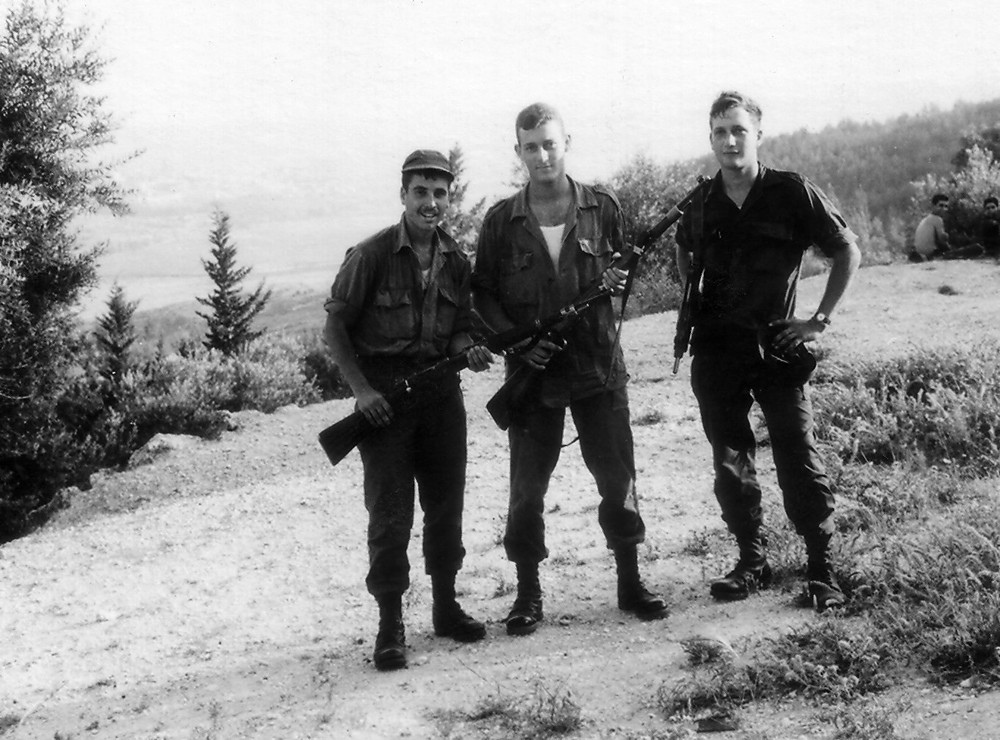
\includegraphics[scale=0.5]{History_Yosya/zoOi_QoHBIM.jpg}
	%	\label{fig:scipion} % Unique label used for referencing the figure in-text\end{document}
	%	%\addcontentsline{toc}{figure}{Figure \ref{fig:placeholder}} % Uncomment to add the figure to the table of contents%----------------------------------------------------------------------------------------
	\caption{Фото с лётного курса, Элиэль в центре. Приблизительно 1970 год. В руках у кадетов — немецкие 98к. Как правило, винтовки были в плохом состоянии, и выдавались военнослужащим тыла — и курсантам-пилотам, к огорчению последних:) Парню справа повезло больше — ему достался «Узи». На втором фото — вручение крыльев. }%	CHAPTER 2
\end{figure}
\begin{figure}[h!tb] 
	\centering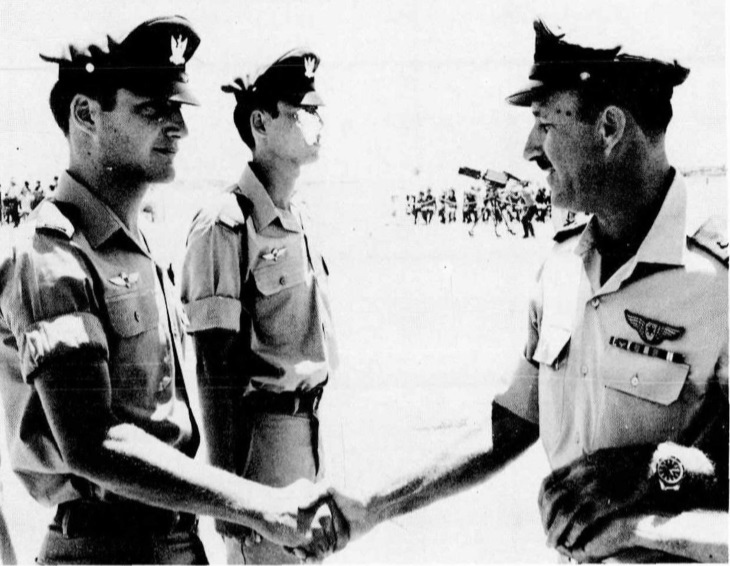
\includegraphics[scale=0.6]{History_Yosya/-t9MlzauznA.jpg}
	%	\label{fig:scipion} % Unique label used for referencing the figure in-text\end{document}
	%	%\addcontentsline{toc}{figure}{Figure \ref{fig:placeholder}} % Uncomment to add the figure to the table of contents%----------------------------------------------------------------------------------------
	\caption{Элиэль получает крылья пилота}%	CHAPTER 2
\end{figure}

В конце 1972 года, после окончания «Курса боевого применения» (фактически, третьего года учебы лётчика в Израиле, когда учат не только летать, но и воевать), он был распределён в 201-ю эскадрилью. Первую эскадрилью «Фантомов» на Святой земле. Такое не было огромной редкостью — просто сразу попасть на «Фантомы» удавалось далеко не всем. Обычно молодые пилоты уходили в эскадрильи «Скайхоков» или старых французских «Самбадов» с «Ураганами», иногда — «Миражей». Но «Фантомы» в качестве первого места службы были не часто. Одним из других молодых пилотов, пришедших в 201-ю из эскадрильи «Самбадов», была Авнер Наве. Его звезда взошла позже, над Ливаном, где он стал первым асом F-15 в мире. Но речь сейчас не о нём.

Настал 1973 год. Война Судного дня. Неожиданная, непонятная, а потому — особенно страшная. Непонятная, потому что арабы вдруг начали побеждать! Страшная — потому, что всю израильскую армейскую вертикаль начала охватывать паника. Под катастрофические сообщения с Голан: «сирийцы идут сквозь нас!» и с южного фронта: «мы потеряли форты на Суэцком канале». В первые дни на эскадрилью Элиэля в буквальном смысле «рухнуло небо» — весь порядок вещей, размеренное планирование каждого шага, уверенность в своём превосходстве не выдержали столкновения с реальностью и утонули в шторме зенитных ракет. Остались без успеха панические попытки заткнуть самолётами огромную «дыру» в оборонительных позициях и вдруг встал непривычный вопрос — что в ВВС Израиля внезапно сломалось? А вдруг они победят?

В первый день войны эскадрилья сбила несколько египетских вертолётов. А во второй случилась самая провальная операция в истории Израиля, «Дугман-5» Из налёта на Голаны не вернулось четыре экипажа. В следующую ночь — гибнут ещё двое. Причем во время совершенно бессмысленной ночной бомбардировке района переправ - лётчики даже толком не знали, где находятся мосты, и бомбили «квадраты» на карте просто чтобы сообщить египтянам, что «фантомы» где-то рядом.

Мораль эскадрильи оказалась близка к опасной черте, когда привычное положение вещей ушло в прошлое. Когда-то советские С-125 смогли сбить два «Фантома» за день, и это было тяжелым ударом для ВВС. Теперь арабы за два дня сбили тринадцать. Трёх дней хватило для того, чтобы началось «выгорание» пилотов. Кто окажется следующим, кто не вернётся в этот раз?

И тогда внезапно выяснилось, что черный юмор может оказаться спасательным кругом. А в этом деле Йосси был большой мастер.

\begin{figure}[h!tb] 
	\centering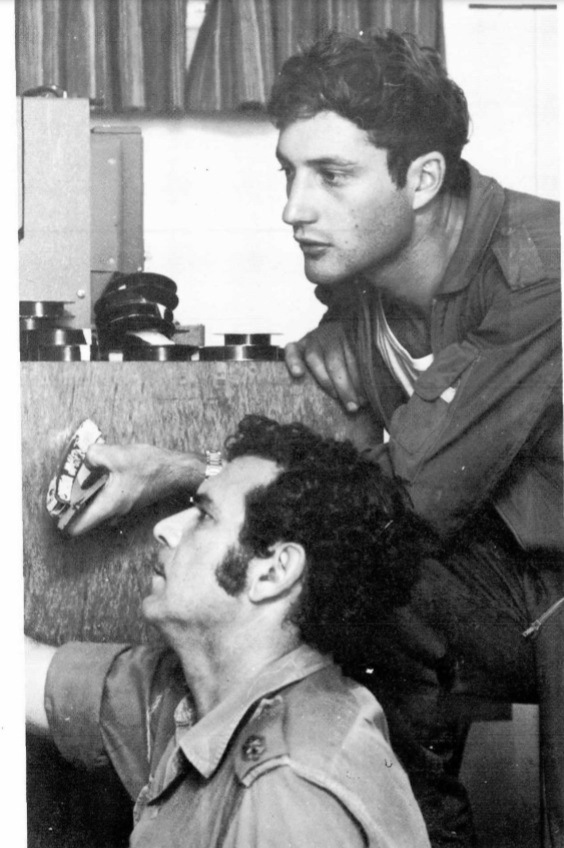
\includegraphics[scale=0.5]{History_Yosya/bJ1O1Q7RhDo.jpg}
	%	\label{fig:scipion} % Unique label used for referencing the figure in-text\end{document}
	%	%\addcontentsline{toc}{figure}{Figure \ref{fig:placeholder}} % Uncomment to add the figure to the table of contents%----------------------------------------------------------------------------------------
	\caption{Пилоты 201 эскадрилья «Фантомов» (верхний — Элиэль) }%	CHAPTER 2
\end{figure}

В один прекрасный день привычную надпись на доске полётных заданий сменило написанное причудливой арабской вязью «добро пожаловать». Такой тонкий намек — дамы и господа, если всё так пойдёт и дальше, то скоро мы все будем разговаривать на другом языке. Самый страшный кошмар обратился в шутку. Йосси приставал к товарищам по эскадрилье с предложением расширить свой запас арабских слов — вдруг в плену пригодится. И вот уже другой кошмар становится смешным. А заодно, одну из старших сержанток эскадрильи из Симы переименовали в Фатьму. Ну а что, тоже весело!

Через много лет сами пилоты вспоминали, что именно такие шутки, черные, злые, на грани фола на удивление сильно поддерживали мораль. Йосси здорово летал, но на земле он сделал гораздо больше, чем в воздухе. В какой-то момент дошло до того, что лётчики эскадрильи пришли к своему комэска и коллективным решением сняли его с должности — на столько сильным было давление. Некоторые пилоты сломались окончательно, но куда меньше, чем могли бы.

А шутки были местами весьма на грани — один из офицеров эскадрильи, чей сын — танкист в то время воевал на Голанах, как-то поделился с Элиэлем своими тревогами о нем. На следующее утро он обнаружил на карте несколько очень больших красных стрелок (обозначавших арабские части) — вокруг подразделения его сына... Элиэля выдал приступ хохота — и вскоре вся эскадрилья имела удовольствие наблюдать, что разозленный офицер по связи с наземными войсками может быть пострашнее сирийских ракет … Элиэль спасся бегством.

\begin{figure}[h!tb] 
	\centering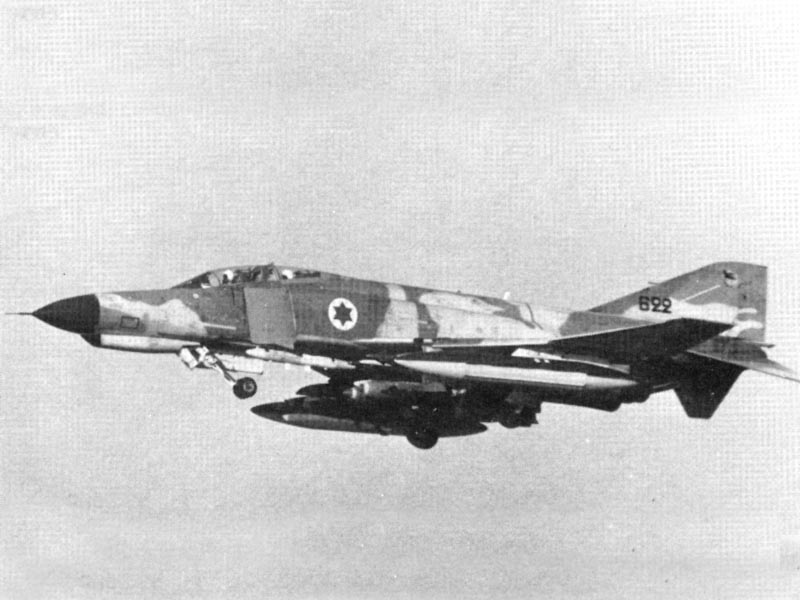
\includegraphics[scale=0.6]{History_Yosya/_bVHHJl_XSk.jpg}
	%	\label{fig:scipion} % Unique label used for referencing the figure in-text\end{document}
	%	%\addcontentsline{toc}{figure}{Figure \ref{fig:placeholder}} % Uncomment to add the figure to the table of contents%----------------------------------------------------------------------------------------
	\caption{"Фантом" 201-й \#622. Рони Хульдаи/Амитай Ицхак сбили египетский Су-7 19 октября 1973}%	CHAPTER 2
\end{figure}

И вот, вся эскадрилья залезает на дерево чёрного юмора. «До встречи в Эль-Меззе (тюрьма в Сирии)», «до встречи на аварийной частоте» — так теперь пилоты провожают друг друга перед вылетами. Один из пилотов ухитрился сказать журналистам — «мы бомбили электростанцию под Дамаском, чтобы наших товарищей перестали пытать электрическим током». Звучит странно - но это сработало, разрядило атмосферу и разгрузило мозг. Несмотря на все потери, на катастрофу начала войны, эскадрилья работала как единый механизм — с первых дней войны до последних. В эскадрилье сменилось три командира — будущего мэра Тель-Авива сменил будущий командир лётной школы, а его будущий главком ВВС. Успешная эскадрилья, во всех смыслах.

201-я бомбила сирийский генштаб в Дамаске, сирийские авиабазы на границе с Турцией, охотилась на сирийские танки в Долине Слёз и египетские в Кантаре и Суэце. Насмерть дралась с «коршунами богини Нехбет» из великолепной египетской 46-й эскадрильи над мостом Банха, когда ошибка командира эскадрильи, Эйтана бен-Элияху стоила им двух экипажей, бомбила «дом египетской истребительной авиации» — авиабазы в Мансуре и Танте (день того боя египтяне объявили днём ВВС). На счету 201-й было больше «Квадратов», чем у любой другой эскадрильи. И больше всего арабских «МиГ-ов».

Элиэль отметился одним сбитым вертолётом - ночью в патрулировании над Офирой с израильских кораблей в Красном море сообщили, что видят над водой египетский Ми-8. Штурман Элиэля захватил цель радаром, получил разрешение и выпустил одну «Спэрроу». Оператор РЛС подтвердил — цель исчезла. С кораблей сообщили — видят попадание, взрыв и множество обломков. Сбитого Элиэлю так и не засчитали — обломков вертолёта так и не смогли найти, средства объективного контроля «фантома» не зафиксировали попадание, а других свидетельств, кроме моряков, не было.

\begin{figure}[h!tb] 
	\centering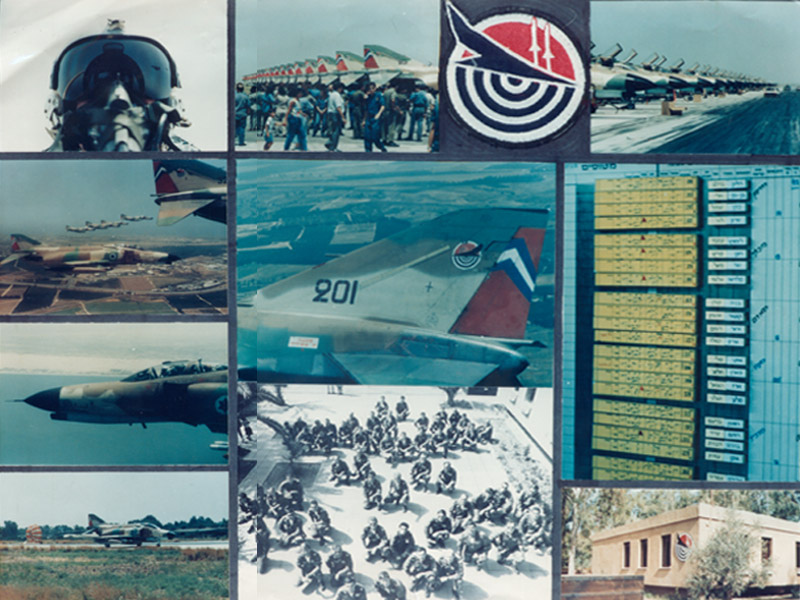
\includegraphics[scale=0.5]{History_Yosya/rcLS8xCibfM.jpg}
	%	\label{fig:scipion} % Unique label used for referencing the figure in-text\end{document}
	%	%\addcontentsline{toc}{figure}{Figure \ref{fig:placeholder}} % Uncomment to add the figure to the table of contents%----------------------------------------------------------------------------------------
	\caption{201-я эскадрилья, фото с сайта http://gal-ed.raanana.muni.il}%	CHAPTER 2
\end{figure}

За пару лет до войны «клоун» Элиэль проявил себя ещё одним очень странным образом. В каждой эскадрилье есть «угол павших», своего рода мини-музей и мемориал. Внезапно, именно Йосси в какой-то момент занялся приведением его в порядок. Посчитал это правильным для себя. Он нашел родственников первого погибшего пилота эскадрильи (его родители давно умерли, нашелся брат), в день памяти собрал на Хатцоре многих родственников других погибших пилотов. А потом с привычными шутками показал на пустое место в углу и сказал — «а это для меня», и засмеялся. Тогда это списали на его специфическое чувство юмора. А кто-то понял, что в этом весёлом циркаче есть что-то более глубокое …

Война закончилась, и Йосси отправился назад в лётную школу. Уже как инструктор. Теперь его боготворили: во-первых, он был ветераном войны, пилотом знаменитой 201-й эскадрильи, и героем в глазах кадетов. Во-вторых, он был весьма хорош собой и в целом имел успех у девушек. А в-третьих (и это самое главное) — он был членом самого закрытого сообщества в ВВС Израиля — пилотажной группы. «Венца славы» лётчика-инструктора.

Группа летала на «Фугах» — учебно-боевых самолётах, на которых производилось обучение пилотов. Как правило, они выступали по большим государственным праздникам — в День независимости, например, выполняя различные сложные фигуры в плотном строю — буквально в метре друг от друга, оставляя за собой шлейфы дыма. С такой лёгкостью и изяществом, что можно было подумать, что это очень легко.

\begin{figure}[h!tb] 
	\centering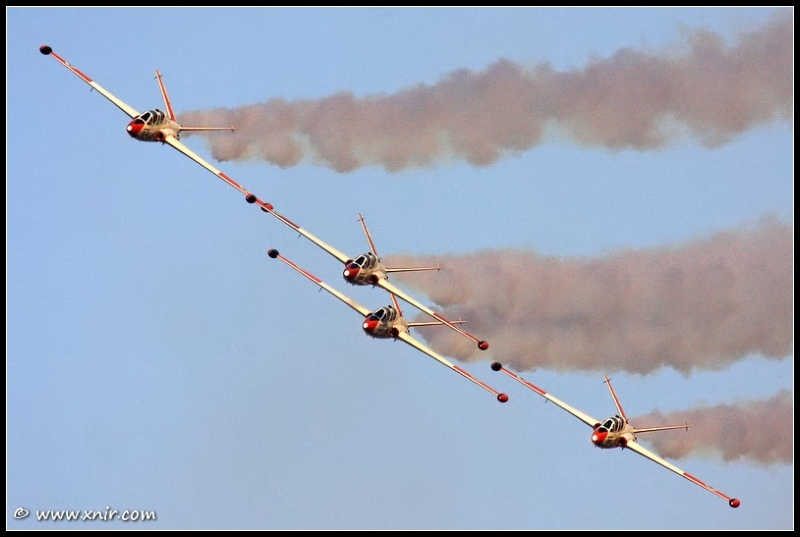
\includegraphics[scale=0.5]{History_Yosya/MiOSXvxzAsk.jpg}
	%	\label{fig:scipion} % Unique label used for referencing the figure in-text\end{document}
	%	%\addcontentsline{toc}{figure}{Figure \ref{fig:placeholder}} % Uncomment to add the figure to the table of contents%----------------------------------------------------------------------------------------
	\caption{«Фуги» пилотажной группы ВВС Израиля. Обратите внимание на расстояние между крыльями.}%	CHAPTER 2
\end{figure}

Элиэль был не только отличным пилотом и красивым парнем. Он действительно умел не только показать, как должна выглядеть фигура пилотажа, но и научить выполнять её правильно. Далеко не все из инструкторов могли этим похвастаться - впрочем, как правило это было проблемой курсантов.

Чувство юмора никуда не делось. Как командир отряда, Элиэль отвечал за программу обучения. Для этого у него была специальная доска, на которой были расписаны планы полётов для каждого курсанта. Причем «отсеянных» оттуда он не стирал. Доступ к кабинету, где стояла доска, для курсантов был закрыт — правда, был один нюанс. Полы в помещениях надо было мыть. Эту тяжелую миссию нередко возлагали на курсантов. Разумеется, «доску Элиэля» они видели — и делились увиденным с товарищами.

Через месяц обучения, когда в рядах курсантов начались серьёзные потери (отсев на «базовом» обучении был порядка 75\%), возле имён отсеянных начали появляться странные значки — чёрточки, звёздочки, крестики. Через некоторое время, такие же значки начали появляться около имён тех, кто остался и продолжал летать. Курсанты сделали единственный возможный вывод, который стоил многим из них бессонных ночей и седых волос. Отсеивание продолжалось, и значки плодились с регулярностью. А Элиэль всё больше улыбался …

Только после окончания этапа обучения, Йосси раскрыл оставшимся секрет — все отметки были не более, чем его розыгрышем. Увидев, что курсанты «подсматривают» (и наверняка делятся наблюдениями) он решил разыграть их, ставя отметки у имён и наблюдая за угрюмой реакцией… Не побили его только потому, что очень уважали как инструктора.

Йосси и в лётной школе иногда летал так, как привык на выступлениях. Тут с ним случалось разное — например, во время одного из полётов с курсантом, он решил «показать класс», и приблизился к другой «Фуге» так, что «бидон» на законцовке крыла оказался буквально в полуметре от кабины. Йосси допустил маленькую ошибку, слишком быстро «взяв ручку» на себя - так, что «бидон» его собственного самолёта ударил хвостовое оперение соседа. Обе покалеченные машины отправились на посадку. Йосси шокировал диспетчера фразой «столкнулся в воздухе, захожу на посадку» — и начал садиться.

Курсант(кстати, он потом стал первым «русским» лётчиком в Израиле) был в шоке — во время посадки до последнего момента было не понятно, что раньше коснётся земли — смятый бидон на крыле, или колесо самолёта. В первом случае самолёт вполне мог «кувыркнуться», и шансов уцелеть было бы не очень много. Впрочем, Элиэль сумел посадить самолёт сначала на правое колесо, а потом, очень бережно, опустить вниз левое. 

\begin{figure}[h!tb] 
	\centering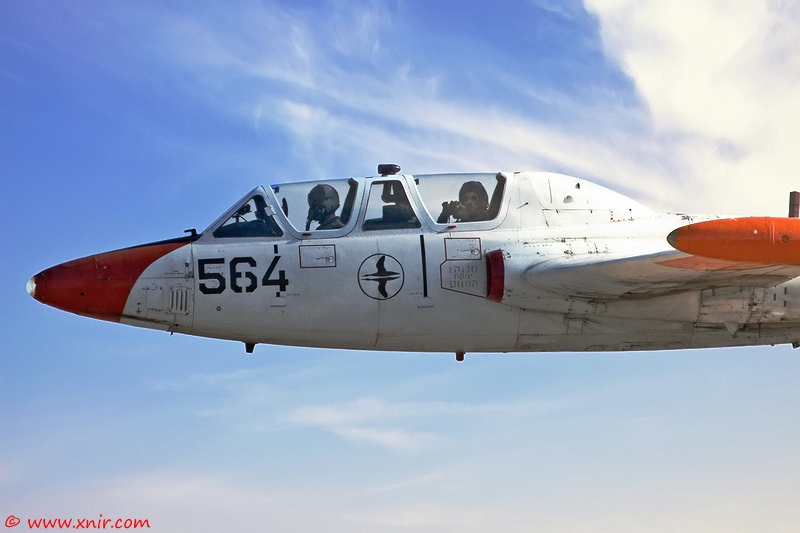
\includegraphics[scale=0.6]{History_Yosya/5YihKMW0Msk.jpg}
	%	\label{fig:scipion} % Unique label used for referencing the figure in-text\end{document}
	%	%\addcontentsline{toc}{figure}{Figure \ref{fig:placeholder}} % Uncomment to add the figure to the table of contents%----------------------------------------------------------------------------------------
	\caption{«Фуги» пилотажной группы ВВС Израиля. Обратите внимание на расстояние между крыльями.}%	CHAPTER 2
\end{figure}

Произошедшее не прошло для него без последствий. Капитан Йоси Элиэль на пол года был дисциплинарно понижен до лейтенанта и отстранён от полётов в аэробатической группе. Последнее было наиболее болезненно.

В пилотажную группу он вернётся чуть больше, чем через год. А ещё через пару лет возглавит её.

В 78-м году Йосси Элиэль женился.

\begin{figure}[h!tb] 
	\centering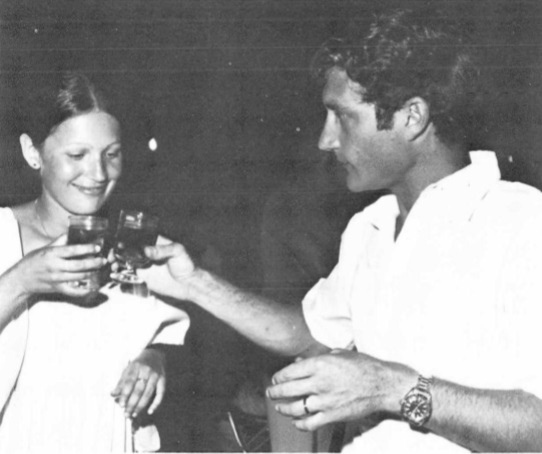
\includegraphics[scale=0.7]{History_Yosya/R9E0MVnKvo4.jpg}
	%	\label{fig:scipion} % Unique label used for referencing the figure in-text\end{document}
	%	%\addcontentsline{toc}{figure}{Figure \ref{fig:placeholder}} % Uncomment to add the figure to the table of contents%----------------------------------------------------------------------------------------
	\caption{Фото с супругой}%	CHAPTER 2
\end{figure}

Примерно тогда-же сослуживцы Йосси написали будущей жене восхитительное письмо, начинавшееся словами:

\textit{«Мы хотели бы дать Анат чуть больше информации о том, что есть что, и особенно - кто есть кто. Другими словами, мы не сомневаемся, что ты хорошо знаешь Элиэля, но позади Джекилла скрывается мистер Хайд, особенно — позади каждого Элиэля... ». }


Пожалуй, это было очень точное описание.

Дальше — как и у многих. «Литани» в 78-м, Первая Ливанская в 82-м. Между ними - многочисленные вылеты против палестинского «гадюшника» в Южном Ливане. Должность замкомэска в эскадрилье «Фантомов». Переподготовка на F-16. После Ливанской войны, отправился в Штаты, учился в Командно-штабном колледже ВВС в Алабаме, получил первую степень в университете Алабамы. Вернулся домой в 83-м, получил подполковника — и 253-ю эскадрилью новейших на тот момент F-16 под командование. Его предшественниками-комэска были легендарные Гиора Эпштейн и Ури Гиль.

И конечно оставалась воздушная акробатика. Не только на «Цукитах» — «Фугах». Теперь в его распоряжении был самый манёвренный боевой самолёт того времени, F-16.

Дальше было ещё больше полётов, и авиашоу. До одного момента …

\textbf{3 июля 1986 года подполковник Йосси Элиэль разбился во время учебно-тренировочного полёта при выполнении фигуры высшего пилотажа на малой высоте, при подготовке программы ко Дню ВВС на глазах у всей авиабазы. Предположительной причиной гибели стала неверная оценка высоты во время выхода из пикирования. На момент гибели ему было 35 лет.}

\begin{textcitation}
	«Дорогая Анат.
	
	Я не могу поверить и не могу осознать горькую новость, что Йосси больше нет с нами.
	
	Его смех, юмор, жизнерадостность, к которым мы привыкли, заставляют меня думать, что это не горькая правда, а очередной его розыгрыш, к которому мы так привыкли.
	
	Мне кажется, что он вернётся завтра и скажет: «хотел посмотреть на ваши грустные лица— а теперь я снова с вами».
	
	Я знал его много лет. Я сопровождал его как инструктор, лидер в пилотажной группе, командир эскадрильи. Я буду сопровождать его в его последнем пути.
	
	Подполковний Йосеф Элиэль погиб 3 июля 1986 года, в учебном полёте, во время опасного упражнения, пытаясь исполнить его наилучшим образом — как обычно. 
	
	Йосси будет скучать по тебе и вашим девочкам, но и нам - всем солдатам авиабазы, лётчикам, командирам - будет его не хватать. Если бы мы могли спросить его, чего бы он хотел, он бы ответил — как всегда, с улыбкой — «жить дальше, летать и оставаться семьёй».
	
	Авием Села
\end{textcitation}

\begin{figure}[h!tb] 
	\centering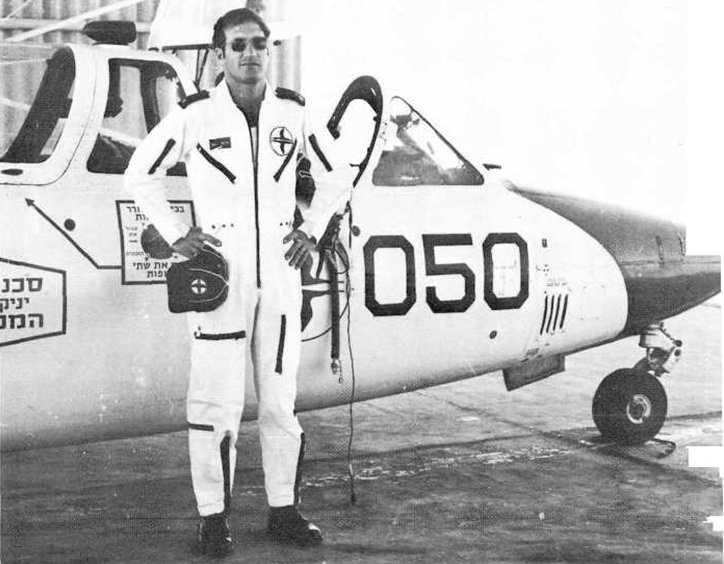
\includegraphics[scale=0.6]{History_Yosya/M8BDQOT5FmA.jpg}
	%	\label{fig:scipion} % Unique label used for referencing the figure in-text\end{document}
	%	%\addcontentsline{toc}{figure}{Figure \ref{fig:placeholder}} % Uncomment to add the figure to the table of contents%----------------------------------------------------------------------------------------
	%	\caption{Фото с супругой}%	CHAPTER 2
\end{figure}

\begin{figure}[h!tb] 
	\centering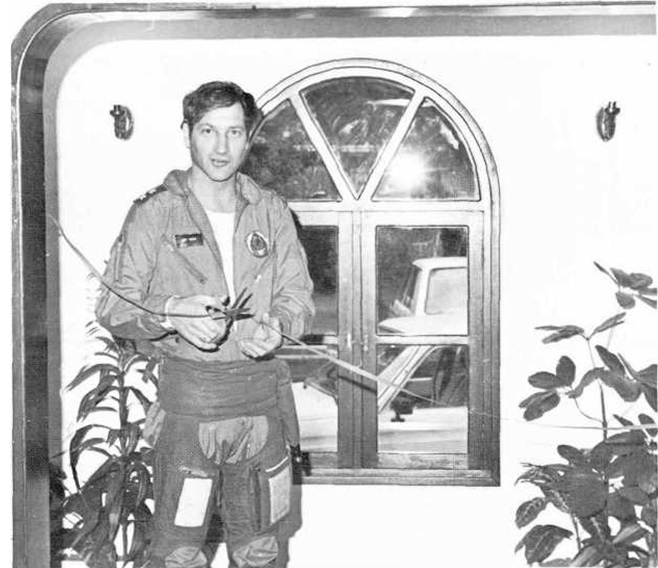
\includegraphics[scale=0.6]{History_Yosya/S960fPX83C8.jpg}
	%	\label{fig:scipion} % Unique label used for referencing the figure in-text\end{document}
	%	%\addcontentsline{toc}{figure}{Figure \ref{fig:placeholder}} % Uncomment to add the figure to the table of contents%----------------------------------------------------------------------------------------
	%	\caption{Фото с супругой}%	CHAPTER 2
\end{figure}
\begin{figure}[h!tb] 
	\centering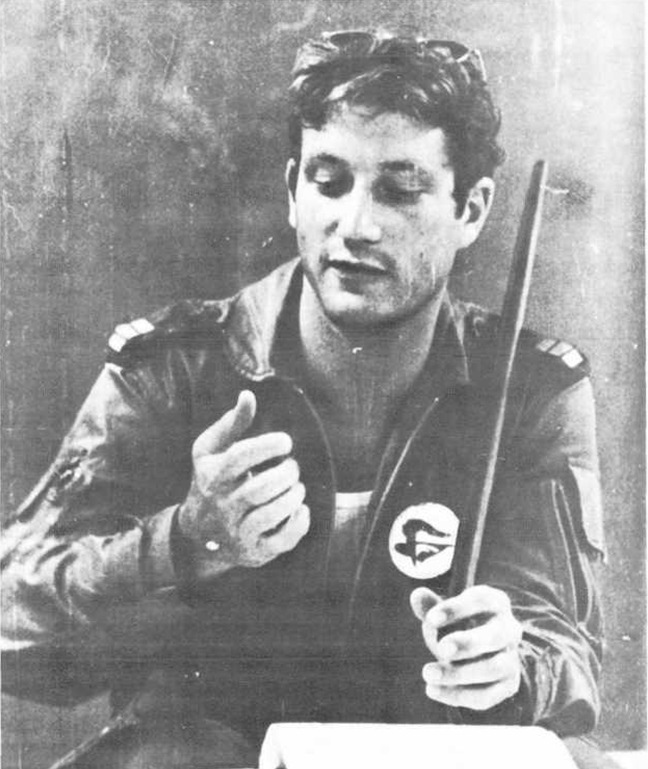
\includegraphics[scale=0.6]{History_Yosya/-KYjwfnSX0E.jpg}
	%	\label{fig:scipion} % Unique label used for referencing the figure in-text\end{document}
	%	%\addcontentsline{toc}{figure}{Figure \ref{fig:placeholder}} % Uncomment to add the figure to the table of contents%----------------------------------------------------------------------------------------
	%	\caption{Фото с супругой}%	CHAPTER 2
\end{figure}

\begin{figure}[h!tb] 
	\centering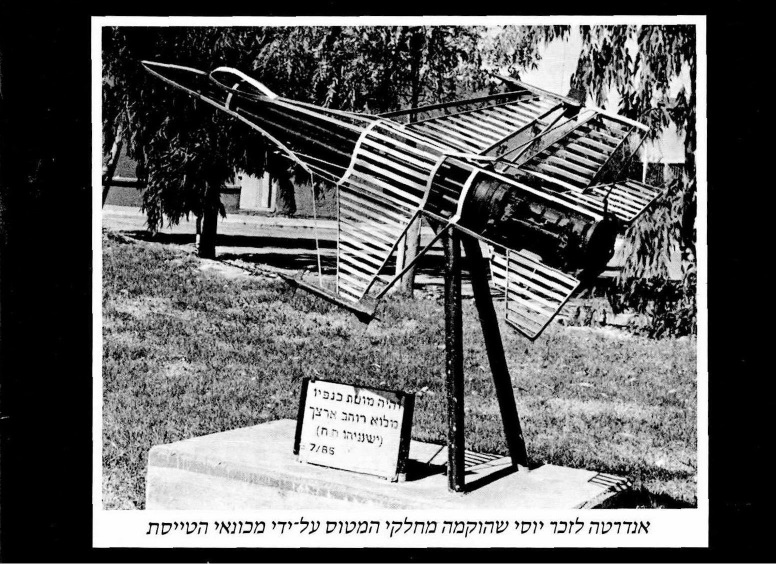
\includegraphics[scale=0.6]{History_Yosya/J3-qpraOxxo.jpg}
	%	\label{fig:scipion} % Unique label used for referencing the figure in-text\end{document}
	%	%\addcontentsline{toc}{figure}{Figure \ref{fig:placeholder}} % Uncomment to add the figure to the table of contents%----------------------------------------------------------------------------------------
	%	\caption{Фото с супругой}%	CHAPTER 2
\end{figure}
\begin{figure}[h!tb] 
	\centering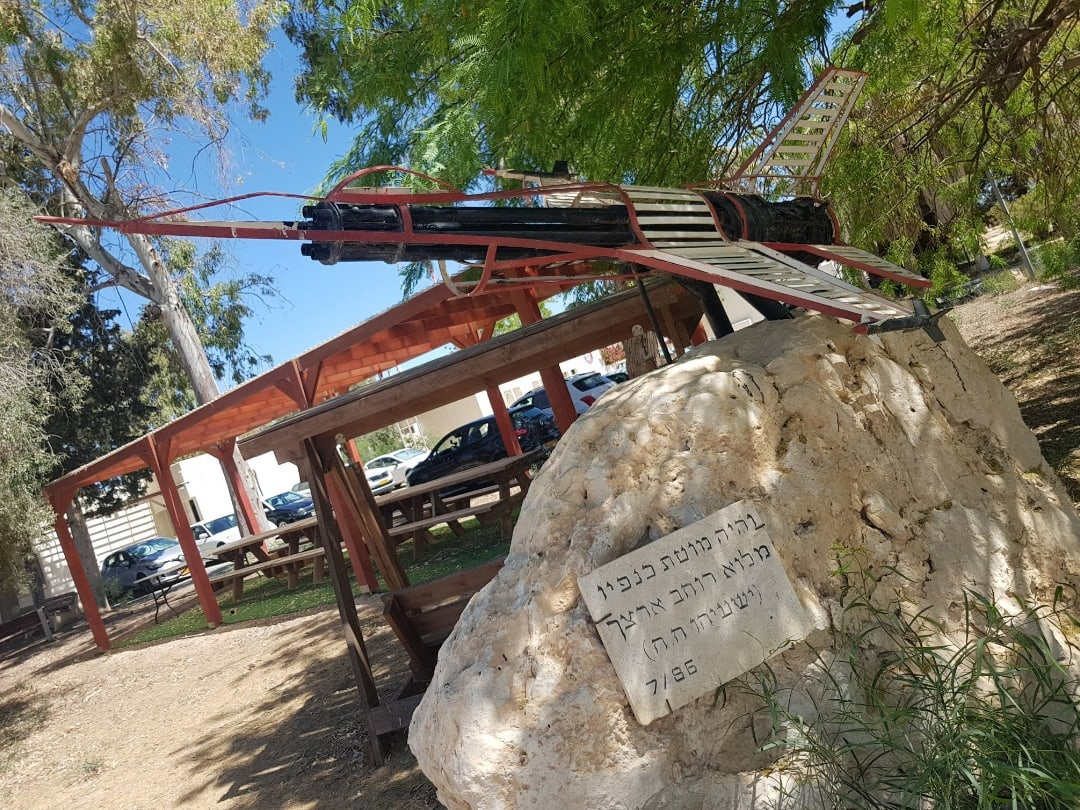
\includegraphics[scale=0.4]{History_Yosya/-O0VmNmFlaU.jpg}
	%	\label{fig:scipion} % Unique label used for referencing the figure in-text\end{document}
	%	%\addcontentsline{toc}{figure}{Figure \ref{fig:placeholder}} % Uncomment to add the figure to the table of contents%----------------------------------------------------------------------------------------
	\caption{Самодельный мемориал Йосси Элиэля в Хацерим.}%	CHAPTER 2
\end{figure}

Использовались источники 
%\cite{barkai, kuper_nikol,mostov,shlomo,segev,israel_vvs,memor_cahal,fisher,raanana,235eskadr}

Фотографии взяты с сайтов https://www.fresh.co.il, и библиотеки института Фишера (www.fisherlibrary.co.il), или сайта ВВС Израиля, если на изображении не указано иное.

К началу \pageref{tablecont}
